\chapter{The most exciting observable}
\label{ch:nedm-at-psi}

\begin{center}
  \emph{Why are we here? Because of CP-symmetry violation.}\\
  prof. Edward Hinds
\end{center}

Symmetry is the most fundamental form of beauty.

The essence of the classical physics are the three symmetries: with respect to the spatial translation (homogeneity of space), with respect to rotation (isotropy of space) and with respect to translation in time (homogeneity of time). Quite literally, as Noether showed, they correspond to the conservation laws of momentum, angular momentum and energy, respectively. By saying the symmetry is conserved, we understand that no physical system becomes any different by \emph{only} having been moved in space, rotated, or looked at later.

These are continuous symmetries. No less fundamental is the triad of symmetries with respect to discrete transformations: $P$, parity transformation, mirroring the spatial dimensions, $T$, time reversal, flipping the arrow of the time, and $C$, charge conjugation, flipping \emph{all} charges of particles. One would expect a beautiful universe to work exactly the same in the mirror, or with matter swapped with anti-matter.

Discrete symmetries can be combined. So $CP$ means a symmetry after flipping the charges \emph{and} mirroring the space. The $CPT$ is a mental refuge: any Lorentz invariant local quantum field theory with a Hermitian Hamiltonian. It scares a humble experimental physicist to think of a theory which would not fulfill this.

Yet, in a perfectly symmetric universe after the Big Bang an equal amount of matter and anti-matter would be created and they would perfectly annihilate. There would not be us.
In 1967 Andrei Sakharov
\marginpar{Andrei Sakharov, pacifist and human-rights activist, was awarded the 1975 Nobel Piece Price, called ``a spokesman for the conscience of mankind''.}
has formulated, that a necessary condition for that not to happen, i.\,e.\ for there to be a bit of matter left over, is a violation of the CP-symmetry.

Physicist have now long accepted violations of the fundamental symmetries.
1956 Chien-Shiung Wu P-violation beta decay of cobalt-60. 
The discovery of CP violation in $K^0_L \rightarrow \pi^+ \pi^-$ decay [1] in 1964 was an amazing event for the majority of theorists
% cite [1] [1] J.H. Christenson, J.W. Cronin, V.L. Fitch, R. Turlay, Phys. Rev. Lett. 13 (1964) 138.
Both have been explained in the scope of the standard model. Complex phases in the quark and neutrino mixing matrices. Theta-QCD.
%\marginpar{An up quark is a mass eigenstate}

Yet, this is not enough. \cite{Pospelov2005} The observed asymmetry is \ldots, while only \ldots can be attributed to the standard model. Despite the SMs tremendous success, we know it is now everything. We \emph{know} that the CP-symmetry is violated somewhere still, but do not know neither where or how. Naturally, we want to find out.

Naturally, many theories have been proposed that offer to solve this, among other, problem. They introduce additional, for that reason, mechanisms of CP-violation. A very popular idea: They introduce additional particles around the scale of weak interactions (several-hundred GeV).

An excellent probe for these theories is the nEDM. is a T-violating, so assuming CPT, also CP-violating observable. Write down the Hamiltonian!
The possibilities are \cite{Ellis1989}.
Also, gives handle on theta-QCD.

\begin{figure}
  \centering
  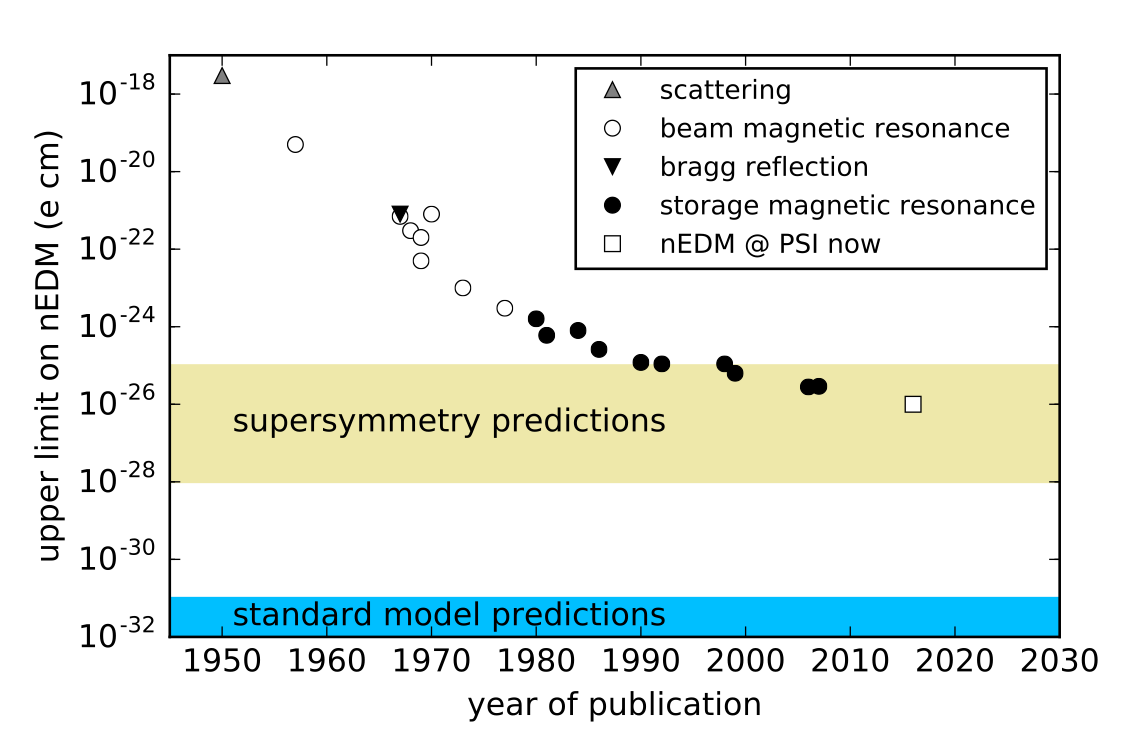
\includegraphics[width=\linewidth]{gfx/introduction/limits.png}
  \caption{\ldots \note{Work it over} \note{Make it BOOOM, state-of-the art, with individual points marked, theories marked, make everyone want to steal it!} \note{If I have the time.}}
  \label{fig:nEDM_limits_history}
\end{figure}

Because it is so sensitive probe for beyond standard model physics, it has been measured since... As a matter of fact, In 1949, before Wu's discovery of P-violation in the weak sector, Purcell and Ramsey performed the measurement to test P-violation in the strong one, using nEDM as the probe. They got zero result. Here explain how they did it! With a figure, not tooo long. The measurement was repeated until \ldots when it was replaced by storage magnetic resonance experiments --- explain briefly the difference.

The last point is the prediction, the author had the honour of being part of it.

